\chapter{Introduction}
\label{ch:introduction}

Nano-satellites have lowered the cost of access to orbit by allowing light payloads to be launched as secondary passengers on heavy-lift rocket flights. However, the cost of the hardware required and the launch itself — when it is not subsidised by the launch provider or space agencies — still limit their use  to well-funded universities and companies.

For applications that require low atmospheric density or medium altitudes, but do not depend on the payload being in a \acrfull{leo}, High-Altitude Balloons (\acrshort{hab}) present an affordable alternative. Such balloons, inflated with low-density gases (usually helium or hydrogen), can reach the stratosphere (altitudes of \SI{30}{\kilo\metre} to \SI{45}{\kilo\metre}). The payload is encased in a thermally insulated container attached under the balloon itself. Depending on the mission, balloons either float at a constant altitude and drift for long durations or climb to the target altitude, then burst under the pressure of the expanding gas. Once the balloon is destroyed, the payload is brought back to the ground under a parachute.

The main component of the payload is the \acrfull{obc}, which controls the different instruments through the different phases of flight (ascent, observation, free-fall and parachute descent). Because high-altitude winds can reach speeds upwards of \SI{150}{\kilo\metre\per\hour} and carry the payload over long distances, most balloons carry a \acrfull{gnss} receiver that the OBC can use to keep track of the balloon's position and altitude. To avoid loosing flight data if the payload is lost or lands in an unaccessible area, the OBC also controls a radio transmission system used to forward payload and ancillary data (\acrshort{gnss} co-ordinates, altitude, systems health) to a ground station as it is acquired.

Depending on the mission, various instruments are added to the payload. The \acrshort{obc} is in charge of gathering, storing and transmitting their data to the ground. Most balloon payloads are designed as custom hardware and software to fit the mission, which means common systems like \acrshort{gnss}, on-board data transfer and radio communications are re-implemented every time.

The satellite industry solves this problem by making use of buses for most missions. Instead of designing a custom, monolithic platform for each new satellite, manufacturers sell buses that provide common utilities (power, data bus, attitude control and platform-to-ground communications) to which the customer or science team connect mission-specific payloads.

\begin{figure}[H]
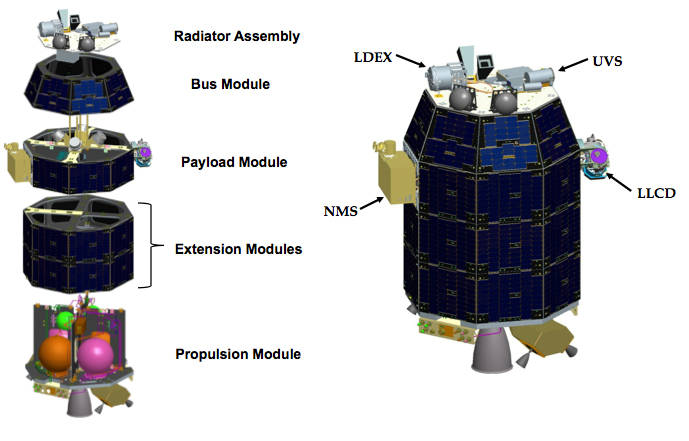
\includegraphics[width=0.35\textwidth]{mcsb.png}
\centering
\caption{LADEE Spacecraft, based on the Modular Common Spacecraft Bus (NASA
Ames)}
\end{figure}

Such modular designs allow mission specialists and scientists to focus on their experiments and payloads, and help reduce cost by spreading common development costs over many missions. Bringing their use to \acrshort{hab} missions would make high-altitude research accessible to a wider range of users, by taking away the computer science and electrical engineering required to design and build the flight computer and radio telemetry system.
\vskip 0.5cm
What are the advantages, issues and obstacles in designing a modular intra-payload and long-range communications platform for \acrlong{hab} scientific missions? The aim of the project presented in this paper was to design, document, implement the protocols, ground and flight software of a low-cost, modular platform to provide data transfer and long-range radio telemetry to payloads carried on \acrlong{hab} missions, and evaluate the prototype's performance. The objectives of the project were:

\begin{itemize}
\item Evaluate existing platforms and protocols used for communications between
payloads and over radio in high-altitude balloons and nano-satellites.

\item Evaluate the feasibility of a modular \acrlong{hab} bus based on low-cost, open-source, off-the-shelf hardware.

\item Design the required protocols and build a prototype for an open-source high-altitude balloon \acrlong{obc} and communication platform.

\item Evaluate the performance of the prototype's payload data bus and radio telemetry system.

\item Evaluate the robustness, maintainability and ease of use of the bus' software compared to that of single-purpose payload firmwares.
\end{itemize}

The project was focused on the software design and implementation of the platform first, and the hardware prototype design second, depending on available resources and time. To limit the scope, the electrical engineering aspect of the proposed platform was not considered past what was required to operate the development boards and the prototype platform. 

The current state of \acrlong{hab} and nano-satellite mission architectures is first discussed in chapter \ref{ch:literature-review}. The proposed platform, \acrshort{ahabus}, and the development process that led to its design are then presented in chapter \ref{ch:methodology}. Finally, chapters \ref{ch:results} and \ref{ch:discussion} present the results of the prototype's testing and show that the project was overall successful, even though more testing will be required to qualify the \acrshort{ahabus} platform for flight.
